This section describes the basic notions of nonabelian topology which I
formalized and applied to higher types in homotopy type theory instead of topological
spaces. Most of the definitions are taken from the book ``Nonabelian
Algebraic Topology'' by Ronald Brown, Philip J. Higgins and Rafael Sivera
\cite{nat}.
The structures used extend classical homotopy theory by considering
\emph{fundamental groupoids} with multiple base points, characterizing the 
interaction between the first and the second homotopy group of a space by 
\emph{crossed modules} as well as \emph{$n$-fold categories}, for which we will
only consider the case $n = 2$.

\section{Double Categories}

%TODO difference to higher categories

To make the precise definition of a double category easier, we observe that we
can define a (small) category $C$ by giving a tuple $(ob_C, hom_C, \partial^-,
\partial^+, \epsilon, \circ_C)$ where
\begin{itemize}
\item $ob_C$ is the set of objects,
\item $hom_C$ is a set that contains all morphisms,
\item $\partial^-$ and $\partial^+ : hom_C \to ob_C$
are maps assigning to each morphism $f$ its domain and codomain,
\item $\epsilon : ob_C \to mor_C$ gives the identity morphism at each element
(this implies $\partial^- \circ_C \epsilon = \partial^+ \circ_C \epsilon = \id$), and
\item $\circ_C$
denotes the composition of morphisms as a partial function $hom_C \times hom_C
\to hom_C$, defined for all $(g, f) \in hom_C \times hom_C$ where
$\partial^+(f) = \partial^-(g)$.
\end{itemize}

In accordance with the geometric interpretation that objects correspond to points while
morphisms correspond to lines we will call $\partial^-$ and $\partial^+$
\textbf{boundary} or \textbf{face maps} while $\epsilon$ will often be referred
to as \textbf{degeneracy map}.

Extending this idea, we want a double category to be an algebraic structure
that does not only contain points and lines but also squares, bounded by four
bounding sides, which we will also call \textbf{faces}.
Like shown in figure \ref{fig:corner-ident}, we must impose conditions on the
face maps so that we can really speak of squares.
Furthermore, just as we needed degenerate lines at each point, we will have
degenerate squares that have a given line at both of their vertical or 
both of their horizontal faces.
In our definiton, $\upperf(u)$, $\lowerf(u)$, $\leftf(u)$ and $\rightf(u)$
will correspond to the upper, lower, left and right face of a square $u$, respectively.
The whole set of faces of a given square $u \in D_2$ will be referred to as
\textbf{shell} of this square.

\begin{figure}[h] \centering
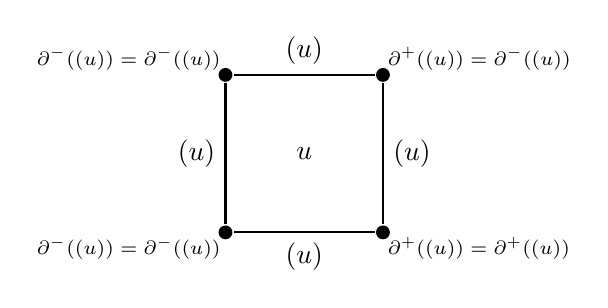
\begin{tikzpicture}[auto,scale=2,color=black,every path/.append style={thick}]
\node(UL) [fill,circle,inner sep=0pt,minimum size=5pt,label={[label distance=-.2cm]above left: 
	{\scriptsize{$\partial^- (\upperf (u)) = \partial^- (\leftf (u))$}}}] at (0,1) {};
\node(UR) [fill,circle,inner sep=0pt,minimum size=5pt,label={[label distance=-.2cm]above right: 
	{\scriptsize{$\partial^+ (\upperf (u)) = \partial^- (\rightf (u))$}}}] at (1,1) {};
\node(BL) [fill,circle,inner sep=0pt,minimum size=5pt,label={[label distance=-.2cm]below left:
	{\scriptsize{$\partial^- (\upperf (u)) = \partial^- (\leftf (u))$}}}] at (0,0) {};
\node(BR) [fill,circle,inner sep=0pt,minimum size=5pt,label={[label distance=-.2cm]below right:
	{\scriptsize{$\partial^+ (\lowerf (u)) = \partial^+ (\rightf (u))$}}}] at (1,0) {};
\draw (UL) -- (UR) node [above, midway] {$\upperf(u)$};
\draw (UR) -- (BR) node [right, midway] {$\rightf(u)$};
\draw (BR) -- (BL) node [below, midway] {$\lowerf(u)$};
\draw (BL) -- (UL) node [left, midway] {$\leftf(u)$};
\node at (0.5,0.5) {$u$};
\end{tikzpicture}
\caption{A square $u \in D_2$, its faces, and its corners.}
\label{fig:corner-ident}
\end{figure}

\begin{defn}[Double category] \label{def:dbl-cat}
A \textbf{double category} $D$ is given by the following data:
Three sets $D_0$, $D_1$, and $D_2$, the elements of which are
respectively called \textbf{0-, 1- and 2-cells}, together with
maps $\partial^-$, $\partial^+$, $\epsilon$, $\circ_D$,
$\partial^-_1$, $\partial^+_1$, $\epsilon_1$, $\circ_1$,
$\partial^-_2$, $\partial^+_2$, $\epsilon_2$, and $\circ_2$
that make these sets form three categories:
\begin{itemize}
\item a category $(D_0, D_1, \partial^-, \partial^+, \epsilon, \circ_D)$ 
on $D_0$, often called the \textbf{(1-)skeleton} of the double category,
\item a \textbf{vertical category}
$(D_1, D_2, \partial^-_1, \partial^+_1, \epsilon_1, \circ_1)$, and
\item a \textbf{horizontal category}
$(D_1, D_2, \partial^-_2, \partial^+_2, \epsilon_2, \circ_2)$.
\end{itemize}

The mentioned maps are required to satisfy the following \textbf{cubical
identities}:
\begin{equation} \label{eq:corner-ident}
\begin{aligned}
\partial^- \circ \partial^-_1 &= \partial^- \circ \partial^-_2\text{,} \\
\partial^- \circ \partial^+_1 &= \partial^+ \circ \partial^-_2\text{,} \\
\partial^+ \circ \partial^-_1 &= \partial^- \circ \partial^+_2\text{,} \\
\partial^+ \circ \partial^+_1 &= \partial^+ \circ \partial^+_2\text{,}
\end{aligned}
\end{equation}
\begin{equation} \label{eq:degen-ident}
\begin{aligned}
\partial^-_1 \circ \epsilon_2 &= \epsilon \circ \partial^-\text{,} \\
\partial^+_1 \circ \epsilon_2 &= \epsilon \circ \partial^+\text{,} \\
\partial^-_2 \circ \epsilon_1 &= \epsilon \circ \partial^-\text{,} \\
\partial^+_2 \circ \epsilon_1 &= \epsilon \circ \partial^+\text{, and}
\end{aligned}
\end{equation}
\begin{equation} \label{eq:zero-unique-ident}
\epsilon_1 \circ \epsilon = \epsilon_2 \circ \epsilon \eqqcolon 0\text{.}	 \\
\end{equation}

The boundary and degeneracy maps of the vertical category are
furthermore assumed to be a homomorphism with respect to
the composition of the horizontal category, and vice versa:
\begin{equation} \label{eq:linear-ident}
\begin{aligned}
\partial^-_2(v \circ_1 u) &= \partial^-_2(v) \circ_D \partial^-_2(u)\text{,} \\
\partial^+_2(v \circ_1 u) &= \partial^+_2(v) \circ_D \partial^+_2(u)\text{,} \\
\partial^-_1(v \circ_2 u) &= \partial^-_1(v) \circ_D \partial^-_1(u)\text{,} \\
\partial^+_1(v \circ_2 u) &= \partial^+_1(v) \circ_D \partial^+_1(u)\text{,} \\
\epsilon_2(g \circ_D f) &= \epsilon_2(g) \circ_1 \epsilon_2(f)\text{, and} \\
\epsilon_1(g \circ_D f) &= \epsilon_1(g) \circ_2 \epsilon_1(g)\text{,}
\end{aligned}
\end{equation}
for each $f, g \in D_1$ and $u, v \in D_2$ where the compositions are defined.

A last condition, called the \textbf{interchange law}, has to be fulfilled:
For each $u, v, w, x \in D_2$,
\begin{equation} \label{eq:interchange}
(x \circ_2 w) \circ_1 (v \circ_2 u) = (x \circ_1 v) \circ_2 (w \circ_1 u)
\end{equation}
has to hold if it is well-defined.
\end{defn}

As seen in figure \ref{fig:corner-ident}, the four identities~(\ref{eq:corner-ident})
correspond to the well-definedness of the corners of a given square $u \in D_2$.
The next four equations~(\ref{eq:degen-ident}) tell us that for any line $f \in D_1$,
besides the identities
$\partial^\pm_1(\epsilon_1(f)) = f$ and
$\partial^\pm_2(\epsilon_2(f)) = f$ (which follow from the definition of a
category), the remaining two faces of a degenerate square are defined as
consisting of the suitable degenerate lines. Figure \ref{fig:degen-ident}
illustrates the cases of both the vertical and the horizontal category.
Equation~(\ref{eq:zero-unique-ident}) is to make sure that in the case where we take the degenerate
square of a line which is itself degenerate, and end up with a square with all four
faces degenerate, it doesn't matter whether we choose the vertical or the horizontal
degeneracy but that instead we receive a unique zero-element for each $x \in D_0$.

\begin{figure} \centering
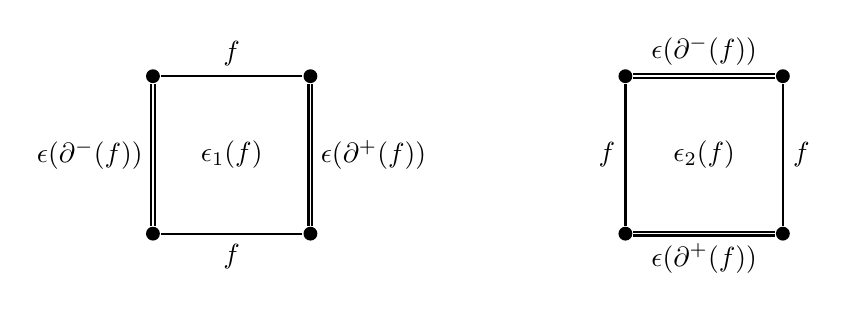
\begin{tikzpicture}[auto,scale=2,color=black,every path/.append style={thick}]
\node(UL) [fill,circle,inner sep=0pt,minimum size=5pt] at (0,1) {};
\node(UR) [fill,circle,inner sep=0pt,minimum size=5pt] at (1,1) {};
\node(BL) [fill,circle,inner sep=0pt,minimum size=5pt] at (0,0) {};
\node(BR) [fill,circle,inner sep=0pt,minimum size=5pt] at (1,0) {};
\draw (UL) -- (UR) node [above, midway] {$f$};
\draw[double] (UR) -- (BR) node [right, midway] {$\epsilon(\partial^+(f))$};
\draw (BR) -- (BL) node [below, midway] {$f$};
\draw[double] (BL) -- (UL) node [left, midway] {$\epsilon(\partial^-(f))$};
\node at (0.5,0.5) {$\epsilon_1(f)$};

\node(UL) [fill,circle,inner sep=0pt,minimum size=5pt] at (3,1) {};
\node(UR) [fill,circle,inner sep=0pt,minimum size=5pt] at (4,1) {};
\node(BL) [fill,circle,inner sep=0pt,minimum size=5pt] at (3,0) {};
\node(BR) [fill,circle,inner sep=0pt,minimum size=5pt] at (4,0) {};
\draw[double] (UL) -- (UR) node [above, midway] {$\epsilon(\partial^-(f))$};
\draw (UR) -- (BR) node [right, midway] {$f$};
\draw[double] (BR) -- (BL) node [below, midway] {$\epsilon(\partial^+(f))$};
\draw (BL) -- (UL) node [left, midway] {$f$};
\node at (3.5,0.5) {$\epsilon_2(f)$};
\end{tikzpicture}
\caption{Degenerate squares of the vertical and horizontal category for a given
line $f \in D_1$. Degenerate lines are drawn as double lines.} %%TODO "double lines"?
\label{fig:degen-ident}
\end{figure}

The linearity condition~(\ref{eq:linear-ident}) serves to define the two faces of
a composite square that are not already fixed by the definition of vertical and
horizontal category.

\begin{figure} \centering
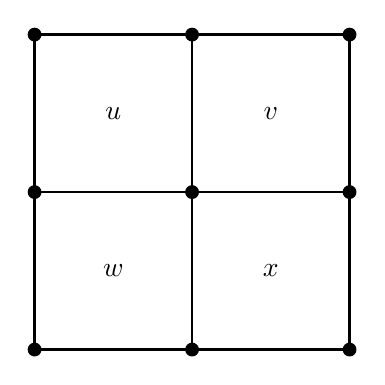
\begin{tikzpicture}[auto,scale=2,color=black,every path/.append style={thick}]
\foreach \x in {0,1,2} {
	\foreach \y in {0,1,2} {
		\node[fill,circle,inner sep=0pt,minimum size=5pt] at (\x,\y) {};
		
	}
	\draw (\x,0) -- (\x,1) -- (\x,2);
	\draw (0,\x) -- (1,\x) -- (2,\x);
}
\node at (0.5,1.5) {$u$};
\node at (1.5,1.5) {$v$};
\node at (0.5,0.5) {$w$};
\node at (1.5,0.5) {$x$};
\end{tikzpicture}
\caption{The grid we use to illustrate the composition $(x \circ_2 w) \circ_1 (v \circ_2 u)$
as well as $(x \circ_1 v) \circ_2 (w \circ_1 u)$, which are identical by the
interchange law.}
\label{fig:interchange}
\end{figure}

The interchange law can be applied to four squares that are composable as a 
$2 \times 2$-grid to another square.
It makes sure that the result of the composition does not depend on whether we
first compose horizontally and then vertically or the other way round.
This justifies illustrating such compositions, as well as larger, iterated ones,
by ``grids'' like the one shown in figure \ref{fig:interchange}.

Starting from a given 1-skeleton, it is easy to find some very simple
but nevertheless very useful and recurring examples for double categories:

\begin{example} \label{def:sq-dbl-cat}
Let $C = (C_0, C_1, \partial^-, \partial^+, \epsilon, \circ_C)$ be a category. The
\textbf{square double category} on $C$ is defined by setting $D_0 \coloneqq C_0$,
$D_1 \coloneqq C_1$ and
\begin{align*}
D_2 \coloneqq \left\{ (f, g, h, i) \right| &\partial^+(f) = \partial^-(i), 
	\partial^+(i) = \partial^+(g), \\ %TODO: Make { bigger
	&\left.\partial^-(g) = \partial^+(h), 
	\partial^-(h) = \partial^-(f) \right\} \subseteq D_1^4
\end{align*}
and $\upperf$, $\lowerf$, $\leftf$, $\rightf$ to be the four projections on
this set. (To keep things consistent, I will always state the faces of a square
in the order upper, lower, left and right.) The degenerate squares are the obvious
quadruples $(f, f, \id, \id)$ and $(\id, \id, f, f)$ for a morphism $f \in C_1$.
Composing two squares $(f, g_1, h_1, i_1)$ and $(g_1, g_2, h_2, i_2)$ vertically
yields a square $(f, g_2, h_2 \circ h_1, i_2 \circ i_1)$.

Note that $f$, $g$, $h$, and $i$ do not have to form a \emph{commutative} square ---
the square double category on $C$ rather collects all possible squares in $C$.
We denote the square double category on $C$ as $\square'C$.
\end{example}

\begin{example} \label{def:shell-dbl-cat}
Let again be $C = (C_0, C_1, \partial^-, \partial^+, \epsilon, \circ_C)$ a category.
We restrict the square double category on $C$ to commutative squares and obtain
the \textbf{commutative square double category} or \textbf{shell double category}
on $C$:
\begin{align*}
D_0 &\coloneqq C_0 \text{,} \\
D_1 &\coloneqq C_1 \text{ and } \\
D_2 &\coloneqq \left\{ (f, g, h, i) \in (\square'C)_2 ~\middle|~ g \circ_C h = i \circ_C f \right\} \text{.}
\end{align*}

Faces and degeneracies are trivial, for defining the the vertical composition of
two squares $(f, g_1, h_1, i_1)$ and $(g_1, g_2, h_2, i_2)$, one obtains the
commutativity of the composed square by
\begin{align*}
g_2 \circ_C h_2 \circ_C h_1 &= i_2 \circ_C g_1 \circ_C h_1 \\
	&= i_2 \circ_C i_1 \circ_C f
\end{align*}
and analogously for the horizontal composition. We write $\square C$ for the
commutative square double category on $C$.
\end{example}

For the purpose of building a category of double categories we have to define what
it means for a map to preserve the structure of a double category:

\begin{defn} \label{def:dbl-functor}
A \textbf{double functor} $F$ between double categories $D$ and $E$ is a triple of maps
$(F_0, F_1, F_2)$ where $F_0 : D_0 \to E_0$, $F_1 : D_1 \to E_1$ and $F_2 : D_2
\to E_2$ such that $(F_0,F_1)$ is a functor between the 1-skeleton of $D$ and $E$
and $(F_1,F_2)$ is a functor between both the vertical and horizontal category
of $D$ and $E$. That means that all faces and degeneracies commute with with $F_1$
resp. $F_2$.
\end{defn}

\begin{lemma} \label{def:cat-of-dbl-cat}
Double functors turn the set of all double categories into a category $\DCat$.
Its initial object is the empty double category, its terminal object consists of the
double category $D$ with $D_0 = D_1 = D_2 = \{\ast\}$.
\hfill $\square$
\end{lemma}
%TODO parts of the proof? pushouts?

\section{Thin Structures and Connections}

We will now enrich double category with even more data: We need a notion of
what it means for a square to be \emph{thin}.
When defining the fundamental double category of a space these thin squares will
correspond to those actual geometric squares inside the considered space, which are
homotopic to degenerate squares. %TODO "which"? "that"?

\begin{defn} \label{def:thin-structure}
Let $D$ be a double category on a category $C = (C_0, C_1)$. Then, a \textbf{thin
structure} on $D$ is a double functor $T : \square C \to D$ which on the 1-skeleton
is the identity.

Equivalently, we can describe a thin structure by marking certain two-cells as
\textbf{thin} in way such that the following hold:
\begin{enumerate}
\item Every commutative shell has a unique thin filler.
\item The horizontal and vertical composition of two thin squares is thin.
\item Degenerate squares are thin.
\end{enumerate}
\end{defn}

In a double category $D$ without a defined thin structure we have
$\epsilon_1(f)$ and $\epsilon_2(f)$ as two ways to receive a square from a given
morphism $f \in D_1$. A thin structure adds two more canonical ways of turning
a line into a square:

\begin{defn} \label{def:connections}
Let $D$ be a double category with a thin structure and $f \in D_1$ a morphism.
Then, the \textbf{lower right connection} of $f$ is the thin square with $f$ 
as its upper and left face and $\epsilon(\partial^+(f))$ as its lower and right face.
Analogously, the \textbf{upper left connection} of $f$ is the thin square with
$f$ on the bottom and right face and $\epsilon(\partial^-(f))$ on the upper and
left side. (See figure \ref{fig:connections}.)
We denote the lower right connection of $f$ with $\Gamma^-(f)$ and the upper left
connection with $\Gamma^+(f)$.
\end{defn}

\begin{figure} \centering
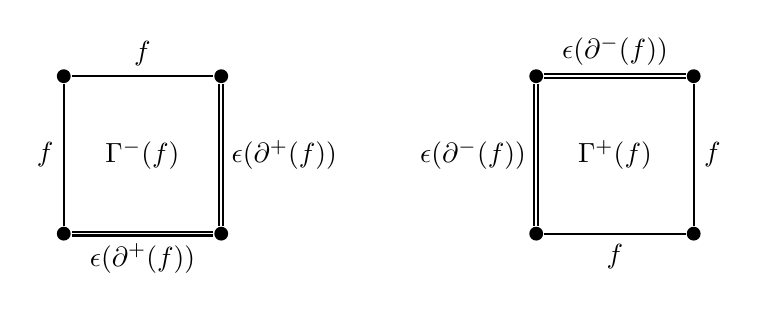
\begin{tikzpicture}[auto,scale=2,color=black,every path/.append style={thick}]
\node(UL) [fill,circle,inner sep=0pt,minimum size=5pt] at (0,1) {};
\node(UR) [fill,circle,inner sep=0pt,minimum size=5pt] at (1,1) {};
\node(BL) [fill,circle,inner sep=0pt,minimum size=5pt] at (0,0) {};
\node(BR) [fill,circle,inner sep=0pt,minimum size=5pt] at (1,0) {};
\draw (UL) -- (UR) node [above, midway] {$f$};
\draw[double] (UR) -- (BR) node [right, midway] {$\epsilon(\partial^+(f))$};
\draw[double] (BR) -- (BL) node [below, midway] {$\epsilon(\partial^+(f))$};
\draw (BL) -- (UL) node [left, midway] {$f$};
\node at (0.5,0.5) {$\Gamma^-(f)$};

\node(UL) [fill,circle,inner sep=0pt,minimum size=5pt] at (3,1) {};
\node(UR) [fill,circle,inner sep=0pt,minimum size=5pt] at (4,1) {};
\node(BL) [fill,circle,inner sep=0pt,minimum size=5pt] at (3,0) {};
\node(BR) [fill,circle,inner sep=0pt,minimum size=5pt] at (4,0) {};
\draw[double] (UL) -- (UR) node [above, midway] {$\epsilon(\partial^-(f))$};
\draw (UR) -- (BR) node [right, midway] {$f$};
\draw (BR) -- (BL) node [below, midway] {$f$};
\draw[double] (BL) -- (UL) node [left, midway] {$\epsilon(\partial^-(f))$};
\node at (3.5,0.5) {$\Gamma^+(f)$};
\end{tikzpicture}
\caption{Lower right and upper left connection of a morphism $f$.} %%TODO "double lines"?
\label{fig:connections}
\end{figure}

We observe that connections are composable in the following sense:

\begin{lemma}[S-laws] \label{thm:s-law}
Let $D$ be a double category with thin structure and $f \in D_1$. Then,
\begin{align*}
\Gamma^-(f) \circ_2 \Gamma^+(f) &= \epsilon_1(f) \text{ and }\\
\Gamma^-(f) \circ_1 \Gamma^-(f) &= \epsilon_2(f) \text{.}
\end{align*}
\end{lemma}

\begin{lemma}[Transport laws] \label{thm:dbl-cat-transport}
Let $D$ be a double category with thin structure and $f, g \in D_1$ with
$\partial^+(f) = \partial^-(g)$. Then,
\begin{align*}
\Gamma^-(g \circ f)
	&= (\Gamma^-(g) \circ_2 \epsilon_2(g)) \circ_1 (\epsilon_1(g) \circ_2 \Gamma^-(f))
	\text{ and } \\
\Gamma^+(g \circ f)
	&= (\Gamma^+(g) \circ_2 \epsilon_1(f)) \circ_1 (\epsilon_2(f) \circ_2 \Gamma^+(f))
	\text{.}
\end{align*}
\end{lemma}
\begin{proof}
As one can easily check (see figures \ref{fig:s-law-horiz} --
\ref{fig:transport-law-plus}) for each of the equations,
the composed squares are well defined and have the faces of the square on the left
hand side coincide with those of the square on the right hand side.
The composite squares are thin because they are a composition of thin squares.
Then, the theorem follows from the uniqueness of thin fillers and the thinness
of identity squares.
\end{proof}

\begin{figure}\centering
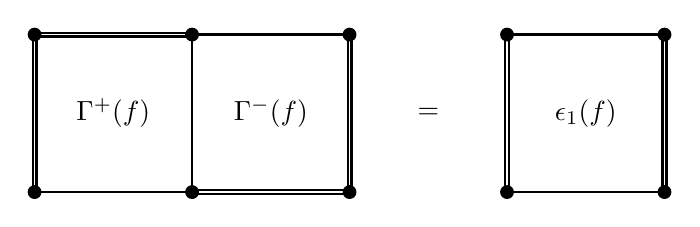
\begin{tikzpicture}[auto,scale=2,color=black,every path/.append style={thick}]
\draw[double] (0,0) -- (0,1) -- (1,1);
\draw[double] (1,0) -- (2,0) -- (2,1);
\draw (0,0) -- (1,0) -- (1,1) -- (2,1);
\draw[double] (3,0) -- (3,1);
\draw[double] (4,0) -- (4,1);
\draw (3,0) -- (4,0);
\draw (3,1) -- (4,1);
\foreach \x in {0,1,2,3,4} {
	\foreach \y in {0,1} {
		\node[fill,circle,inner sep=0pt,minimum size=5pt] at (\x,\y) {};
	}
}
\node at (2.5,0.5) {$=$};
\node at (0.5,0.5) {$\Gamma^+(f)$};
\node at (1.5,0.5) {$\Gamma^-(f)$};
\node at (3.5,0.5) {$\epsilon_1(f)$};
\end{tikzpicture}
\caption{The horizontal S-law.}
\label{fig:s-law-horiz}
\end{figure}

\begin{figure} \centering
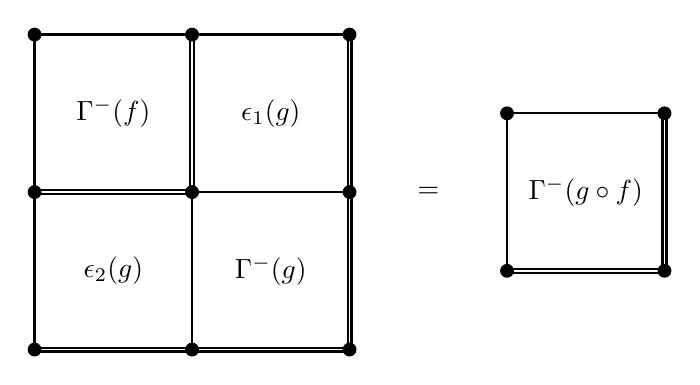
\begin{tikzpicture}[auto,scale=2,color=black,every path/.append style={thick}]
\draw[double] (0,0) -- (2,0) -- (2,2);
\draw[double] (0,1) -- (1,1) -- (1,2);
\draw (0,0) -- (0,2) -- (2,2);
\draw (1,0) -- (1,1) -- (2,1);
\foreach \x in {0,1,2} {
	\foreach \y in {0,1,2} {
		\node[fill,circle,inner sep=0pt,minimum size=5pt] at (\x,\y) {};
		
	}
}
\node at (0.5,1.5) {$\Gamma^-(f)$};
\node at (1.5,1.5) {$\epsilon_1(g)$};
\node at (0.5,0.5) {$\epsilon_2(g)$};
\node at (1.5,0.5) {$\Gamma^-(g)$};
\node at (2.5,1) {$=$};
\draw[double] (3,0.5) -- (4,0.5) -- (4,1.5);
\draw (3,0.5) -- (3,1.5) -- (4,1.5);
\node[fill,circle,inner sep=0pt,minimum size=5pt] at (3,0.5) {};
\node[fill,circle,inner sep=0pt,minimum size=5pt] at (4,0.5) {};
\node[fill,circle,inner sep=0pt,minimum size=5pt] at (3,1.5) {};
\node[fill,circle,inner sep=0pt,minimum size=5pt] at (4,1.5) {};
\node at (3.5,1) {$\Gamma^-(g \circ f)$};
\end{tikzpicture}
\caption{The transport law for $\Gamma^-(g \circ f)$.}
\label{fig:transport-law-minus}
\end{figure}

\begin{figure} \centering
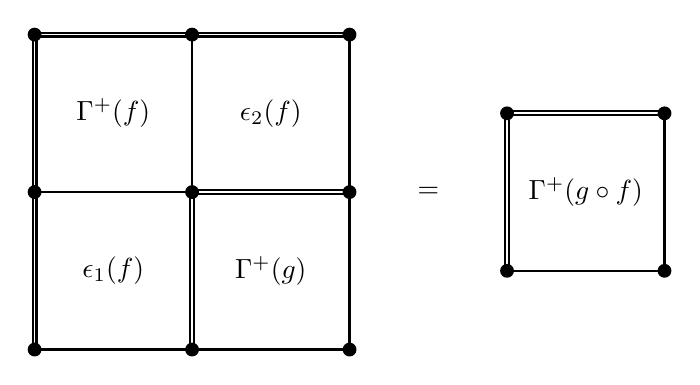
\begin{tikzpicture}[auto,scale=2,color=black,every path/.append style={thick}]
\draw (0,0) -- (2,0) -- (2,2);
\draw (0,1) -- (1,1) -- (1,2);
\draw[double] (0,0) -- (0,2) -- (2,2);
\draw[double] (1,0) -- (1,1) -- (2,1);
\foreach \x in {0,1,2} {
	\foreach \y in {0,1,2} {
		\node[fill,circle,inner sep=0pt,minimum size=5pt] at (\x,\y) {};
		
	}
}
\node at (0.5,1.5) {$\Gamma^+(f)$};
\node at (1.5,1.5) {$\epsilon_2(f)$};
\node at (0.5,0.5) {$\epsilon_1(f)$};
\node at (1.5,0.5) {$\Gamma^+(g)$};
\node at (2.5,1) {$=$};
\draw (3,0.5) -- (4,0.5) -- (4,1.5);
\draw[double] (3,0.5) -- (3,1.5) -- (4,1.5);
\node[fill,circle,inner sep=0pt,minimum size=5pt] at (3,0.5) {};
\node[fill,circle,inner sep=0pt,minimum size=5pt] at (4,0.5) {};
\node[fill,circle,inner sep=0pt,minimum size=5pt] at (3,1.5) {};
\node[fill,circle,inner sep=0pt,minimum size=5pt] at (4,1.5) {};
\node at (3.5,1) {$\Gamma^+(g \circ f)$};
\end{tikzpicture}
\caption{The transport law for $\Gamma^+(g \circ f)$.}
\label{fig:transport-law-plus}
\end{figure}

\section{Double Groupoids}

In general, paths in topological spaces are non-oriented or can be reversed.
Our algebraic structures describing paths and squares should reflect this behavior
by the property that also its morphisms and two-cells should be reversible.
Categories $C$ in which for each morphism $f \in C_1$ there exists an inverse
$f\inv \in C_1$ are called \emph{groupoids}. We apply this concept not only
to the 1-skeleton but also to the two-cells of a
double category, which can be inverted vertically as well as horizontally.

\begin{defn} \label{def:weak-dbl-gpd}
A \textbf{weak double groupoid} is a double category $D$ where all three categories
--- the 1-skeleton, the vertical category and the horizontal category --- are
groupoids. The inverses of a square $u \in D_2$ in the vertical and horizontal category 
will be denoted by $\invv$ and $\invh$ and can be seen as flipping the square
along horizontal, resp. vertical, line.

For a double category to be a \textbf{double groupoid} we further require it to
come with a fixed thin structure.
\end{defn}

Note, that the three notions of inversion interact with each other by yielding
the following laws:

\begin{lemma}[Coherence of inverses] \label{thm:dbl-gpd-inv} %TODO
Let $D$ be a weak double groupoid, $a \in D_1$ and $u \in D_2$. Then,
\begin{equation} \label{eq:inv-coherence1}
\begin{aligned}
\epsilon_1(a) \circ_2 \epsilon_1(a\inv)
	&= \epsilon_2(a) \circ_1 \epsilon_2(a\inv)
	= 0(\partial^-(a)) \text{,} \\
\epsilon_1(a\inv) \circ_2 \epsilon_1(a)
	&= \epsilon_2(a\inv) \circ_1 \epsilon_2(a)
	= 0(\partial^+(a)) \text{,}
\end{aligned}
\end{equation}

\begin{equation} \label{eq:inv-coherence2}
\begin{aligned}
\upperf(\invh(u)) &= \upperf(u)\inv \text{,} \\
\lowerf(\invh(u)) &= \lowerf(u)\inv \text{,} \\
\leftf(\invv(u)) &= \leftf(u)\inv \text{,} \\
\rightf(\invv(u)) &= \rightf(u)\inv \text{,}
\end{aligned}
\end{equation}

\begin{equation} \label{eq:inv-coherence3}
\begin{aligned}
\epsilon_1(a\inv) &= \invh(\epsilon_1(a)) \text{, and } \\
\epsilon_2(a\inv) &= \invv(\epsilon_2(a)) \text{.}
\end{aligned}
\end{equation}
\end{lemma}

\begin{proof}
All equations follow
from the fact that the face maps and degeneracies are homomorphic and thus also
respect inverses.
\end{proof}

We can furthermore prove that our intuition is right assuming that horizontally
inverting the vertical composition of squares is equal to composing the inverted
squares:

\begin{lemma}[Distributivity of inverses] For a weak double groupoid $D$ and
$v, u \in D_2$ the following equations hold as soon as they are well defined:
\begin{equation} \label{eq:inv-distrib}
\begin{aligned}
\invv(v \circ_2 u) &= \invv(v) \circ_2 \invv(u) \text{ and } \\
\invh(v \circ_1 u) &= \invh(v) \circ_1 \invh(u) \text{.}
\end{aligned}
\end{equation}
\end{lemma}

\begin{proof}
We only prove the first equation since the second one results from transposition
of the situation and is provable analogously.
Using the previous calculations and the interchange law we see that
\begin{align*}
(\invv(v) \circ_2 \invv(u)) \circ_1 (v \circ_2 u)
= 	& (\invv(v) \circ_1 v) \circ_2 (\invv(u) \circ_1 u) \\
= 	& \epsilon_1(\upperf(v)) \circ_2 \epsilon_1(\upperf(u)) \\
=	& \epsilon_1(\upperf(v) \circ \upperf(u)) \\
=	& \epsilon_1(\upperf(v \circ_2 u)) \\
=	& \invv(v \circ_2 u) \circ_1 (v \circ_2 u) \text{.}
\end{align*}
Cancelling out $v \circ_2 u$ gives the desired result.
\end{proof}

Observing that we can ``rotate'' a square by 180 degrees in two ways, by first
taking the vertical and then the horizontal inverse or vice versa, we can prove
that those are actually one and the same:

\begin{lemma} \label{thm:rotate-180}
For any weak double groupoid $D$ and square $u \in D_2$,
\begin{equation*}
\invv(\invh(u)) = \invh(\invv(u)) \text{.}
\end{equation*}
\end{lemma}

\begin{proof}
Similar to the last proof we calculate that
\begin{align*}
\invv(\invh(u)) \circ_2 \invv(u)
	&= \invv(\invh(u) \circ_2 u) \\
	&= \invv(\epsilon_2(\leftf(u))) \\
	&= \epsilon_2(\leftf(u)\inv) \\
	&= \invh(\invv(u)) \circ_2 \invv(u) \text{.}
\end{align*}
\end{proof}

%TODO S-lemmas
Of course, the two basic examples we saw for double categories extend to
double groupoids:
\begin{lemma}[Square and shell double groupoids] \label{thm:shell-dbl-gpd}
If C is a groupoid, then the square double category $\square' C$ and the
shell double category $\square C$ are double groupoids.
\end{lemma}

\begin{proof}
It is easily seen for both cases that $\invv(f, g, h, i) \coloneqq (g, f, h\inv, i\inv)$
and $\invh(f, g, h, i) \coloneqq (f\inv, g\inv, i, h)$ provide valid inverses.
Thin squares in both double categories are exactly those in $(\square C)_2$,
which makes $\square C$ a double groupoids with all squares thin. %TODO a "thin double gpd"?
\end{proof}

We will now take a look at the most important example of a double groupoid:
The fundamental double groupoid of a triple of spaces. 
It extends and generalizes the definition of the fundamental group and the second
homotopy group of a space.
We start by extending the idea of the set of loops based at a point by allowing
multiple base points and adding squares.
Just like its classical homotopy theoretic counterpart,
the following structure does \emph{not} already define a double groupoid until we
quotient out homotopy classes.

\begin{defn}[Filtered maps] \label{def:filtered-maps}
Let $C \subseteq A \subseteq X$ be a nested triple of topological spaces.
We obtain sets of points, lines and squares by defining
\begin{itemize}
\item $R(X, A, C)_0 \coloneqq C$,
\item $R(X, A, C)_1 \coloneqq \left\{ \sigma : (I, \partial I) \to (A, C) \right\}$, and
\item $R(X, A, C)_2 \coloneqq \left\{ \alpha : (I^2, \partial I^2, \partial^2 I^2)
	\to (X, A, C) \right\}$, where
\end{itemize}
the maps are meant to be \emph{based} in the sense that they should map the
components of the indicated tuples to their counterparts.
In other words, the points in $R(X, A, C)$ are the points in $C$ , the lines
are paths in $A$ with endpoints located in $C$ and the two-cells are squares
in $X$ which have faces in $A$ and corners in $C$.

Note that $R(X, A, C)_1$ in the case of $C = \{ \ast \}$ becomes the loop space
based in $\ast$ and in the case of $C = A = \{ \ast \}$ the elements of
$R(X, A, C)_2$ end up to be maps $\mathbb{S}^2 \to X$ based in $\ast$.

Just as for a double groupoid we give faces, degeneracies, compositions
and inversions. They might seem familiar from classical homotopy theory
since they are just an extension of the operation that defines the loop group:

For a line $\sigma : (I, \partial I) \to (A , C)$, the left and right face are
simply given by $\sigma(0)$ and $\sigma(1)$. For a square $\alpha$ we define
$\upperf(\alpha)(x) = \alpha(0,x)$, $\lowerf(\alpha)(x) = \alpha(1,x)$,
$\leftf(\alpha)(x) = \alpha(x,0)$ and $\rightf(\alpha)(x) = \alpha(x,1)$.

Degenerate lines are constant maps $I \to C$, degenerate squares $\alpha$ are
those where $\alpha(x,y) = \sigma(x)$ or $\alpha(x,y) = \sigma(y)$ for some
line $\sigma$.

Composition of two composable squares $\alpha$ and $\beta$ is defined analogously
to the composition of paths in the loop group:
\begin{align*}
(\beta \circ_1 \alpha) &= \begin{dcases*}
	\alpha(2x,y) & if $0 \leq x \leq \frac{1}{2}$, \\
	\beta(2x-1,y) & if $\frac{1}{2} \leq x \leq 1$ as well as
	\end{dcases*} \\
(\beta \circ_2 \alpha) &= \begin{dcases*}
	\alpha(x,2y) & if $0 \leq y \leq \frac{1}{2}$, \\
	\beta(x,2y-1) & if $\frac{1}{2} \leq y \leq 1$.
	\end{dcases*}
\end{align*}
Inversion is given by $\sigma\inv(x) = \sigma(1-x)$ for a line $\sigma$ and
$\invv(\alpha)(x,y) = (1-x,y)$, $\invh(\alpha)(x,y) = (y,1-x)$ for a square
$\alpha$.
\end{defn}

The next step is to define the fundamental double groupoid of a triple of
spaces by modding out equivalence classes of filtered maps:

\begin{defn}
We define the \textbf{fundamental double groupoid} $\Pi_2(X, A, C)$ of a nested
triple of spaces $C \subseteq A \subseteq X$ by defining
\begin{align*}
\Pi_2(X, A, C)_0 &\coloneqq C \text{,}\\
\Pi_2(X, A, C)_1 &\coloneqq R(X,A,C)_1 / \equiv \text{, and} \\
\Pi_2(X, A, C)_2 &\coloneqq R(X,A,C)_2 / \equiv \text{,}
\end{align*}
where in the first case $\equiv$ denotes homotopy rel vertices meaning that two
paths $\sigma$ and $\sigma'$ are equivalent iff there is a homotopy
$H : I^2 \to A$ that leaves both endpoints fixed:
\begin{equation*}
\forall t \in I : H(t,0) = H(0,0) \in C \text{ and } H(t,1) = H(0,1) \in C \text{.}
\end{equation*}
For the squares, $\equiv$ we also require the considered homotopies 
$H : I^3 \to X$ to keep the corners fixed.
But more, we require the homotopies \emph{thin} in the sense that for all
$x \in \partial I^2$ we have $H(t,x) \in A$ for all $t \in I$.

It can easily be seen that the operations defined on squares and lines in
definition \ref{def:filtered-maps} respect this definition of equivalence and that
the resulting structure is, indeed, a weak double groupoid.

This is furthermore the point where the reason for the name ``thin structure'' becomes
clear:
To define a thin structure on $\Pi_2(X, A, C)$ we put the predicate ``thin''
on those equivalence classes of squares that contain a squre $\alpha : I^2 \to X$
where $\alpha(x, y) \in A$ for all $x, y \in I$.
It is obvious that this property is closed under the composition of squares and
it is true by definition that for all $\sigma \in \Pi_2(X, A, C)_1$ the condition
is fulfilled for $\epsilon_1(\sigma)$ and $\epsilon_2(\sigma)$.

If for lines $f, g, h, i : I \to A$ we have $g \circ h = i \circ f$ in
$\Pi_2(X, A, C)$, there is a homotopy $H : I^2 \to A$ rel vertices between
$g \circ h$ and $i \circ f$.
It is true that in this case we can also choose $H$ such that $f$, $g$, $h$, and
$i$ lie on the four faces of a square.
We define such a choice of $H$ to be our thin filler for that quadruple of faces.
%TODO: prove this, even if brown doesn't

As a last step we have to prove that this choice is unique up to thin homotopy.
We assume that we are not only given a thin square $H$ for
lines $f$, $g$, $h$, and $i$ but also another thin square $H'$ for a set of lines
$f'$, $g'$, $h'$, $i'$, respectively equivalent to $f$, $g$, $h$ and $i$.
To see that $H$ and $H'$ can be ``connected'' with a thin homotopy,
we consider them, and the homotopies $H_g$, $H_h$, and $H_i$ between three of the faces,
as five faces of a a cube:

\begin{center}
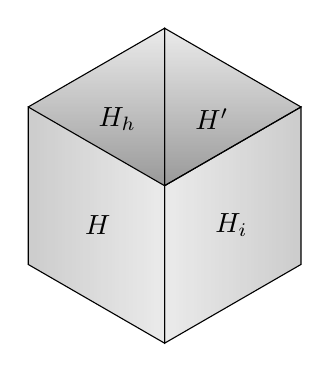
\begin{tikzpicture}
\shade[top color=gray!20, bottom color=gray!100,opacity=0.8,scale=2] (0,0) -- (30:1) -- (0,1) -- (0,0);
\shade[top color=gray!20, bottom color=gray!100,opacity=0.8,scale=2] (0,0) -- (0,1) -- (150:1);
\shade[left color=gray!50, right color=gray!20,opacity=0.8,scale=2] (0,0) -- (0,-1) -- (210:1) --(150:1)--(0,0);
\shade[left color=gray!20, right color=gray!50,opacity=0.8,scale=2] (0,0) -- (30:1) -- (-30:1) --(0,-1)--(0,0);
\draw[scale=2] (0,0) -- (30:1) -- (0,1) -- (0,0);
\draw[scale=2] (0,0) -- (0,1) -- (150:1);
\draw[scale=2] (0,0) -- (0,-1) -- (210:1) --(150:1)--(0,0);
\draw[scale=2] (0,0) -- (30:1) -- (-30:1) --(0,-1)--(0,0);
\node at (-.85,-.5) {$H$};
\node at (.85,-.5) {$H_i$};
\node at (-.6,.85) {$H_h$};
\node at (.6,.85) {$H'$}; %TODO: make this a better picture
\end{tikzpicture}
\end{center}

We can fill this cube and receive a thin homotopy $I^3 \to X$ by simply choosing
a point $p$ above the cube and mapping each point in $I^3$ to its image under the
projection onto the box centered in $p$.
\end{defn}

Before we move on to introduce another algebraic structure that is useful for
the analysis of the first and second homotopy group of a space, here is an example
for a space and its fundamental double groupoid:

\begin{example}[The fundamental double groupoid of the sphere] \label{example:fdblgpd-sphere}
Let $X \coloneqq \mathbb{S}^2$ be the 2-sphere, $A \subset X$ its equator and
$C = \{c_1, c_2, c_3, c_4\} \subset A$ four points on the equator (see
figure \ref{fig:fund-dbl-gpd-sphere}).

Then, $\Pi_2(X, A, C)$ has $C$ as point set, lines are generated by the segments
$\overline{c_0 c_1}$, $\overline{c_1 c_2}$, $\overline{c_2 c_3}$ and
$\overline{c_3 c_4}$.
All two-cells are the result of composition of the upper and lower hemisphere
and degenerate squares on the equator.
\end{example}

\begin{figure} \centering
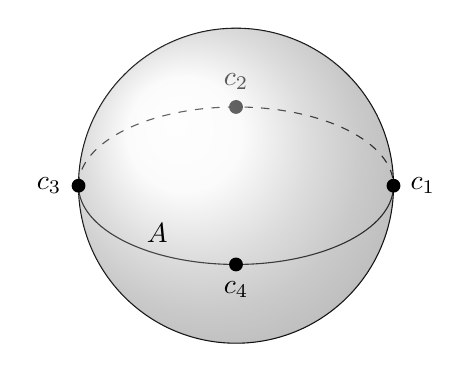
\begin{tikzpicture}[scale=2]
\draw (-1,0) arc (180:360:1 and 0.5);
\draw[dashed] (-1,0) arc (180:0:1 and 0.5);
\draw (0,0) circle (1);
\node [fill,circle,inner sep=0pt,minimum size=5pt,label=above:$c_2$	] at (0,0.5) {};
\shade[ball color=gray!10!white,opacity=0.40] (0,0) circle (1);
\node [fill,circle,inner sep=0pt,minimum size=5pt,label=right:$c_1$] at (1,0) {};
\node [fill,circle,inner sep=0pt,minimum size=5pt,label=left:$c_3$] at (-1,0) {};
\node [fill,circle,inner sep=0pt,minimum size=5pt,label=below:$c_4$] at (0,-0.5) {};
\node at (-0.5,-0.3) {$A$};
%\node at (0.3,0) {$C$};
\end{tikzpicture}
\caption{Filtered presentation of the sphere.}
\label{fig:fund-dbl-gpd-sphere}
\end{figure}

\begin{defn}[Category of double groupoids]
Since morphisms between groupoids are nothing but functors between their underlying
categories we can, without changing the definition of morphisms, enhance our
category $\DCat$ of double categories to a \textbf{category of weak double groupoids}.
This category is thus a full subcategory of $\DCat$.

But to a greater degree we are interested in the \textbf{category of double
groupoids} : This is the category $\DGpd$ containing as objects all double groupoids
and as morphisms all double functors that preserve the attached thin structure in
the sense that they map thin squares to thin squares.

\end{defn}

\section{Crossed Modules}

\begin{figure} \centering
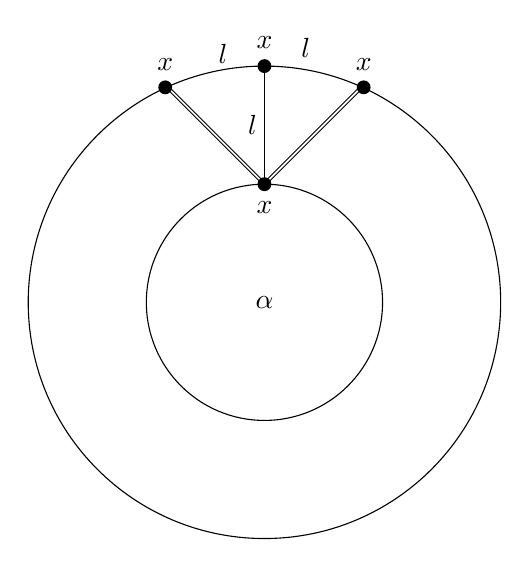
\begin{tikzpicture}[scale=1.5]
\draw (0,0) circle (1);
\draw (0,0) circle (2);
\draw (0,1) -- (0,2);
\begin{scope} \clip (0,0) circle (2);
	\draw[double] (0,1) -- (-2,3);
	\draw[double] (0,1) -- (2,3);
\end{scope}
\node at (0,0) {$\alpha$};
\node [fill,circle,inner sep=0pt,minimum size=5pt,label=below:$x$] at (0,1) {};
\node [fill,circle,inner sep=0pt,minimum size=5pt,label=above:$x$] at (0,2) {};
\node [fill,circle,inner sep=0pt,minimum size=5pt,label=above:$x$] at (0.84,1.82) {};
\node [fill,circle,inner sep=0pt,minimum size=5pt,label=above:$x$] at (-.84,1.82) {};
\node at (-.1,1.5) {$l$};
\node at (-.35,2.1) {$l$};
\node at (.35,2.15) {$l\inv$}; %TODO improve this drawing
\end{tikzpicture}
\caption{Pasting a loop $l$ to a disk $\alpha$.}
\label{fig:xmod-motivation}
\end{figure}


%TODO: cite whitehead
The motivation to introduce crossed modules as a tool for the analysis of the
homotopy properties of a topological space comes from observing that in the
long exact sequence of relative homotopy groups for the constellation 
$x \in A \subseteq X$,
the second relative homotopy group $\pi_2(X, A, x)$ and the fundamental group
$\pi_1(A, x)$ of the subspace are related in the following two ways:
\begin{enumerate}
\item There is a boundary map $\pi_2(X, A, x) \to \pi_1(A, x)$ which is induced
by mapping a representative $\alpha : (\mathbb{D}^2, \partial \mathbb{D}^2) \to 
(X, A)$ to its restriction to the boundary $\left.\alpha\right|_{\partial \mathbb{D}^2}
: \mathbb{S}^1 \to A$.
\item The group $\pi_1(A, x)$ acts on $\pi_2(X, A, x)$ by ``glueing'' the
representative $l$ of $\pi_1(A, x)$ on the disk that represents the given
element $[\alpha] \in \pi_2(X, A, x)$.
We receive the resulting disk by extending $\alpha$ in a degenerate way along
$l$ as illustrated in figure \ref{fig:xmod-motivation}.
\end{enumerate}
These two means of interaction can furthermore be observed to fulfil more algebraic
requirements that will be captured in the definition of a crossed module:
\begin{itemize}
\item The boundary of a representative which was created by pasting $l \in \pi_1(A, x)$
to a disk $[\alpha] \in \pi_2(X, A, x)$ is the
concatenation of paths $l\inv \cdot \partial \alpha \cdot l$.
\item The disk resulting from pasting the boundary of a disk $\beta \in \pi_2(X, A, x)$
to a disk $\alpha \in \pi_2(X, A, x)$ is homotopic to the composition
$\beta\inv \cdot \alpha \cdot \beta$ in $\pi_2(X, A, x)$.
\end{itemize}
So the boundary map and the action resemble the \emph{conjugation} of group elements
in two different ways. This motivates bundling these properties into a new algebraic
structure:

\begin{defn}[Crossed module over a group]
Let $P$ be a group. A \textbf{crossed module} on $P$ is another group $M$ together
with a group homomorphism $\mu : M \to P$ and a group action $\phi$ of $P$ on
$M$ such that:
\begin{enumerate}
\item For all $a \in P$, $x \in M$:
\begin{equation} \label{eq:gp-CM1}
\mu(\phi(a,x)) = a \cdot \mu(x) \cdot a\inv \text{.} %TODO should the \invr really be on the right side?
\end{equation}
\item For all $x, c \in M$ :
\begin{equation} \label{eq:gp-CM2}
\phi(\mu(c),x) = c \cdot x \cdot c\inv \text{.}
\end{equation}
\end{enumerate}
\end{defn}

Crossed modules are not only motivated by geometric examples but also used to
capture a very common, purely group theoretic configuration:

\begin{example}[Normal subgroup crossed module]
Let $G$ be a group and $N \subseteq G$ a normal subgroup of $G$. Then $N$ is made a
crossed module on $G$ by the inclusion map $i : N \to G$ and the conjugation action
of $G$ on $N$.
\end{example}
%TODO talk about computations on xmod/g
%TODO more easy examples

Now we are not interested in the absolute and relative homotopy groups based in
one point but want to adapt the structure to fit well to the concept of fundamental
\emph{groupoids} instead of fundamental groups.
This obvious choice to achieve this is, unsurprisingly, to replace the base group $P$ in
the definition of a crossed module by a groupoid:

\begin{defn}[Crossed module over a groupoid] \label{def:xmod-gpd}
Let $P$ be a groupoid.
A \textbf{crossed module} over $P$ is a group $M_p$
for every $p \in P$ together with
with a family of group homomorphisms $(\mu_p : M_p \to \hom_P(p,p))_{p \in P}$
and a map $\phi$ which is a \emph{groupoid action} of $P$ on $M$ in the sense that
it maps a pair $(a,x)$, where $a \in \hom_P(p,q)$ and $x \in M_p$, to an element
of $M_q$, such that $\phi(\id_p,x) = x$, $\phi(b \circ_P a, x) = \phi(b,(\phi(a,x))$
and $\phi(a, y \cdot_{M_p} x) = \phi(a,y) \cdot_{M_q} \phi(a,x)$ for all
$p, q, r \in P, x,y \in M_p, a \in \hom_P(p,q)$ and $b \in \hom_P(q,r)$.

And, just in the case of crossed modules over a group, we require $\mu$ and $\phi$
to fulfil the following two essential equations:
\begin{enumerate}
\item For all $a \in \hom_P(p,q)$ and $x \in M_p$:
\begin{equation} \label{eq:gp-CM1}
\mu_q(\phi(a,x)) = a \circ \mu_p(x) \circ a\inv \in \hom_P(q,q) \text{.}
\end{equation}
\item For all $c, x \in M_p$ :
\begin{equation} \label{eq:gp-CM2}
\phi(\mu_p(c),x) = c \cdot x \cdot c\inv \in M_p \text{.}
\end{equation}
\end{enumerate}
\end{defn}

With this definition we can extend the example from the beginning of this
chapter by allowing not only $x$ as an endpoint of the paths considered but every
point in a set $C \subseteq A$.
This generalization results in the definition of the \textbf{fundamental crossed
module} of a triple of spaces $C \subseteq A \subseteq X$.

To make the set of crossed module a category, we need to define what a morphism
between two crossed modules should be:

\begin{defn}[Morphisms between crossed modules]
Let $(M_p)_{p \in P}$ be a crossed module over a groupoid $P$, with homomorphism
$\mu$ and action $\phi$ and let $(N_q)_{q \in Q}$ be a crossed module over $Q$
with morphism $\mu'$ and action $\phi'$.
A \textbf{morphism} between $(M_p)_{p \in P}$ and $(N_q)_{q \in Q}$ is a functor $F$
between $P$ and $Q$ and a family of group homomorphisms $(\psi_p)_{p \in P}$ 
with $\psi_p : M_p \to N_{F(p)}$ such that %TODO check if there's more conditions
\begin{itemize}
\item $F \circ \mu_p = \mu'_{F(p)} \circ \psi_p$ for all $p \in P$ and
\item for all $p, q : P$, $a \in \hom_P(p,q)$ and $x : M_p$, the action is preserved:
\begin{equation*}
\psi_q(\phi(a,x)) = \phi(F(a),\psi_p(x)) \text{.} %TODO: double check this
\end{equation*}
\end{itemize}
\end{defn}

\begin{defn}[Category of crossed modules]
All crossed modules on groupoids form a category $\XMod$ using the previously
defined morphisms. Crossed modules over groups are a full subcategory of $\XMod$.
\end{defn}

\section[DGpd and XMod are Equivalent]{Double Groupoids and Crossed Modules are Equivalent}

Comparing the fundamental crossed module and the fundamental double groupoid we
observe that these two structures contain basically the same information.
In fact, not only those particular examples do, but we can prove that the categories
$\DGpd$ and $\XMod$ are equivalent.

In this chapter, the functors $\gamma : \DGpd \to \XMod$ and
$\lambda : \XMod \to \DGpd$ will be presented as well as a proof that $\gamma \lambda$
and $\lambda \gamma$ are naturally isomorphic to the respective identity functors.

\begin{lemma}[The crossed module associated to a double groupoid]
Let $G$ be a double groupoid. We set
\begin{align*}
P &\coloneqq (G_0,G_1) \text{ and } \\
M_p &\coloneqq \left\{ u \in G_2 \middle| \lowerf(u) = \leftf(u) = \rightf(u) = \epsilon(p) \right\}
	\text{ for $p \in G_0$.}
\end{align*}
Then, $M_p$ is a group with composition $\circ_2$, neutral element $0(p)$ and
inverse $\invh$.
Let further be $\mu = \upperf$ and let $\phi(a,u) =
\epsilon_1(a) \circ_2 u \circ_2 \epsilon_1(a\inv) \in M_q$ for $a \in \hom_P(p,q)$
and $u \in M_p$.

The given data $P$, $(M_p)_{p \in P}$, $\mu$ and $\phi$ form a crossed module $\gamma G$.
\end{lemma}

\begin{figure} \centering
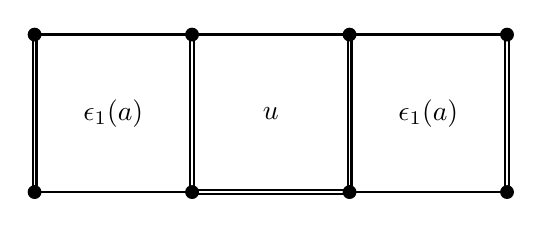
\begin{tikzpicture}[auto,scale=2,color=black,every path/.append style={thick}]
\draw[double] (0,0) -- (0,1);
\draw[double] (1,1) -- (1,0) -- (2,0) -- (2,1);
\draw[double] (3,0) -- (3,1);
\draw (0,1) -- (3,1);
\draw (0,0) -- (1,0);
\draw (2,0) -- (3,0);
\foreach \x in {0,1,2,3} {
	\foreach \y in {0,1} {
		\node[fill,circle,inner sep=0pt,minimum size=5pt] at (\x,\y) {};
	}
}
\node at (0.5,0.5) {$\epsilon_1(a\inv)$};
\node at (1.5,0.5) {$u$};
\node at (2.5,0.5) {$\epsilon_1(a)$};
\end{tikzpicture}
\caption{The result $\phi(a,u)$ of a morphism $a \in \hom_P(p,q)$ acting
on a two-cell $u \in M_p$ three of whose faces are degenerate.}
\label{fig:gamma-phi}
\end{figure}

\begin{proof}
We easily check that $\mu(\phi(a,u)) = a \circ u \circ a\inv$ for any $u \in M_p$
and $a \in hom_P(p,q)$.
To see, that $\phi(\mu_p(c),u) = c \circ_2 u \circ_2 c\inv$ for $u,c \in M_p$,
we consider the composite square
\begin{equation*}
\left(c \circ_2 0(p) \circ_2 \invh(c)\right) \circ_1
	\left(\epsilon_1(\upperf(c)) \circ_2 u \circ_2 \upperf(c\inv)\right) \text{,}
\end{equation*}
which, when evaluated as is, resolves to $\phi(\mu_p(c),u)$, but after applying
the interchange law twice becomes
\begin{equation*}
\left(c \circ_1 \epsilon_1(\upperf(c))\right)
	\circ_2 \left(0(p) \circ_1 u\right)
	\circ_2 \left(\invh(c) \circ_1 \upperf(c\inv)\right)
\end{equation*}
and can be simplified to $c \circ_2 u \circ_2 c$ (see figure \ref{fig:gamma-cm2}).
\end{proof}

\begin{defn}
The construction of $\gamma G$ can be extended to a map from double functors to
morphisms of crossed modules and we obtain a functor $\gamma : \DGpd \to \XMod$.
\end{defn}

\begin{figure} \centering
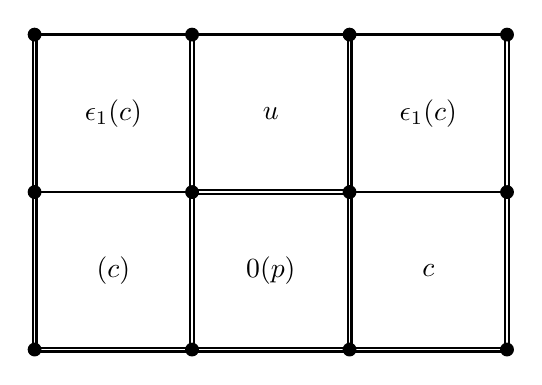
\begin{tikzpicture}[auto,scale=2,color=black,every path/.append style={thick}]
\draw[double] (0,2) -- (0,0) -- (3,0) -- (3,2);
\draw[double] (1,2) -- (1,0);
\draw[double] (2,2) -- (2,0);
\draw[double] (1,1) -- (2,1);
\draw (0,1) -- (1,1);
\draw (0,2) -- (3,2);
\draw (2,1) -- (3,1);
\foreach \x in {0,1,2,3} {
	\foreach \y in {0,1,2} {
		\node[fill,circle,inner sep=0pt,minimum size=5pt] at (\x,\y) {};
	}
}
\node at (0.5,1.5) {$\epsilon_1\upperf(c\inv)$};
\node at (1.5,1.5) {$u$};
\node at (2.5,1.5) {$\epsilon_1\upperf(c)$};
\node at (0.5,0.5) {$\invh(c)$};
\node at (1.5,0.5) {$0(p)$};
\node at (2.5,0.5) {$c$};
\end{tikzpicture}
\caption{A composite square proving the second crossed module axiom for $\gamma G$.}
\label{fig:gamma-cm2}
\end{figure}

But how can we recover a double groupoid given a crossed module on a groupoid?

\begin{lemma}[The double groupoid associated to a crossed module]
Let $(M_p)_{p \in P}$ be a crossed module on a groupoid $P$. We define
\begin{equation*}
G_2 \coloneqq \left\{ (f,g,h,i,m) \middle| 
	\mu(m) = i \circ f \circ h\inv \circ g\inv \right\} \text{.}
\end{equation*}
Then, $G_2$ forms the set of two cells of a double groupoid $\lambda (P, (M_p))$
with the first four projections as face maps.
\end{lemma}

\begin{proof}
Defining the vertical composition of squares $u = (f, g_1, h_1, i_1, m)$ and
$v = (g_1, g_2, h_2, i_2, n)$ as $v \circ_1 u \coloneqq 
(f, g_2, h_2 \circ h_1, i_2 \circ i_2, \phi(i_2, m) \cdot n)$ is well-defined
since
\begin{align*}
\mu(\phi(i_2,m) \cdot n) &= i_2 \circ \mu(m) \circ i_2\inv \circ \mu(n)\\
	&= i_2 \circ i_1 \circ f \circ h_1\inv \circ g_1\inv \circ
		i_2\inv \circ i_2 \circ g_1 \circ h_2\inv \circ g_2\inv \\
	&= (i_2 \circ i_1) \circ f \circ (h_2 \circ h_1)\inv \circ g_2\inv
\end{align*}
and the horizontal composition of $u = (f_1, g_1, h, i_1, m)$ and
$v = (f_2, g_2, i_1, i_2, n)$ likewise by $v \circ_2 \coloneqq
(f_2 \circ f_1, g_2 \circ g_1, h, i_2, n \cdot \phi(g_2,m))$ with
\begin{align*}
\mu(n \cdot \phi(g_2,m)) &= \mu(n) \circ g_2 \circ \mu(m) \circ g_2\inv \\
	&= i_2 \circ f_2 \circ i_1\inv \circ g_2\inv \circ g_2 \circ
		i_1 \circ f_1 \circ h\inv \circ g_1\inv \circ g_2\inv \\
	&= i_1 \circ (f_2 \circ f_1) \circ h \circ (g_2 \circ g_1)\inv
\end{align*}
Identity squares are given by $(f,f,\epsilon(p),\epsilon(q),1)$ and
$(\epsilon(p),\epsilon(q),f,f,1)$ for $f \in \hom_P(p,q)$. Identity and
associativity laws follow easily from the fact that $\phi$ respects identity
morphisms as well as the composition in $M_p$ and in $P$.
\end{proof}

\begin{defn}
The map $\lambda$ can be turned into a functor $\lambda : \XMod \to \DGpd$ by
extending it to morphisms of crossed modules.
\end{defn}

We conclude this chapter by stating:
\begin{thm}
The categories $\DGpd$ and $\XMod$ are equivalent.
\end{thm}

\begin{proof}
We show that there are isomorphic natural transfromations $\gamma \lambda \simeq \id_{\XMod}$
and $\lambda \gamma \simeq \id_{\DGpd}$.

These transformation are just the identity on points an morphisms so we only have
to consider their definition on two-cells.
For a crossed module $(M_p)_{p \in P}$,
\begin{align*}
\gamma(\lambda(M_p)) &= \left\{ (f,g,h,i,m) ~\middle|~
	\mu(m) = i \circ f \circ h\inv \circ g\inv, g = h = i = \id_p \right\} \\
	&= \{ (f, \id_p, \id_p, \id_p, m) ~|~ \mu(m) = f\} \\
	&\cong M_p \text{.}
\end{align*}
It is easy to check that this isomorphism of groups extends to an isomorphism
of crossed modules and that it is natural in $(M_p)_{p \in P}$.

To find a suitable natural isomorphism $\lambda \gamma \simeq \id_{\DGpd}$,
we have to match the structure of two-cells in a double groupoid, which are
compsable in two dimensions, to the one-dimensional nature of a group.
\end{proof}

%\section{The 2-dimensional Seifert-van Kampen theorem for spaces}











